%%%%%%%%%%%%%%%%%%%%%%%%%%%%%%%%%%%%%%%%%%%%%%%%%%%%%%%%%%%
\documentclass[xcolor=x11names,compress]{beamer}
%\documentclass[xcolor=x11names,compress, handhouts, aspectratio=169]{beamer}
%% General document
\usepackage{graphicx, subfig}
%% Beamer Layout
\useoutertheme[subsection=false,shadow]{miniframes}
\useinnertheme{default}
\usefonttheme{serif}
\usepackage{palatino}

%%%%%%% Mes Packages %%%%%%%%%%%%%%%%
%\usepackage[french]{babel}
\usepackage[T1]{fontenc}
\usepackage{color}
\usepackage{xcolor}
\usepackage{dsfont} % Pour indicatrice
\usepackage{url}
\usepackage{multirow}
\usepackage[normalem]{ulem}   % For strike out text

% Natbib for clean bibliography
\usepackage[comma,authoryear]{natbib}

%remove the icon
\setbeamertemplate{bibliography item}{}

%remove line breaks
\setbeamertemplate{bibliography entry title}{}
\setbeamertemplate{bibliography entry location}{}
\setbeamertemplate{bibliography entry note}{}

%% ------ MEs couleurs --------
\definecolor{vert}{rgb}{0.1,0.7,0.2}
\definecolor{brique}{rgb}{0.7,0.16,0.16}
\definecolor{gris}{rgb}{0.7, 0.75, 0.71}
\definecolor{twitterblue}{rgb}{0, 0.42, 0.58}
\definecolor{airforceblue}{rgb}{0.36, 0.54, 0.66}
\definecolor{violet}{RGB}{112,48,160}
\definecolor{orange}{RGB}{233,113,50}
\definecolor{siap}{RGB}{3,133, 200}





%%%%%%%%%%%%%%%%% BEAMER PACKAGE %%%%%%%

\setbeamercolor{itemize item}{fg=siap}
%\setbeamercolor{itemize subitem}{fg=blue}
%\setbeamercolor{itemize subsubitem}{fg=cyan}

\setbeamerfont{title like}{shape=\scshape}
\setbeamerfont{frametitle}{shape=\scshape}

\setbeamercolor*{lower separation line head}{bg=DeepSkyBlue4}
\setbeamercolor*{normal text}{fg=black,bg=white}
\setbeamercolor*{alerted text}{fg=siap}
\setbeamercolor*{example text}{fg=black}
\setbeamercolor*{structure}{fg=black}
\setbeamercolor*{palette tertiary}{fg=black,bg=black!10}
\setbeamercolor*{palette quaternary}{fg=black,bg=black!10}

% Set the header color to SIAP's color
\setbeamercolor*{frametitle}{fg=siap}

%remove navigation symbols
\setbeamertemplate{navigation symbols}{}

\renewcommand{\(}{\begin{columns}}
\renewcommand{\)}{\end{columns}}
\newcommand{\<}[1]{\begin{column}{#1}}
\renewcommand{\>}{\end{column}}

%% Add footer with logo
\setbeamertemplate{footline}{%
  \begin{beamercolorbox}[wd=\paperwidth,ht=2.5ex,dp=1.125ex,%
    leftskip=.3cm,rightskip=.3cm plus1fil]{author in head/foot}
    
\includegraphics[height=4ex]{SIAP_logo_2020_1800.png}\hfill
    \insertshortauthor\hfill\insertshorttitle\hfill  \textcolor{siap}{\textit{\insertframenumber}}
  \end{beamercolorbox}%
}

% Path for the graphs
\graphicspath{
{Graphics/}
{c:/Chris/UN-ESCAP/SIAP-E-learning/Resources/OpenScience/}
{c:/Chris/UN-ESCAP/MyCourses2023/RAP/Slides/Graphics/}
{c:/GitMain/RAP/RAP-Course/images/}
{c:/GitMain/RAP/RAP-Course/images/logos/}
% Path for specific graphs created
 }


\title[\textcolor{siap}{Principles of RAP}]{\textcolor{siap}{Principles of \\ Reproducible Analytical Pipelines \\}
\vspace{0.55cm} \textcolor{brique}{What's next?}}
\author{Christophe Bontemps}
\institute{\large{\emph{Statistical Institute for Asia and the Pacific} } \\
    
\includegraphics[height=10ex]{SIAP_logo_2020_1800.png}}
\date{}


\begin{document}

\begin{frame}
\titlepage
\end{frame}


\section{Full Reproducibility}

\begin{frame}
\frametitle{Towards \emph{full} reproducibility }
There are many other things to control for \emph{full} reproducibility:
\begin{columns}[t]
 \begin{column}{0.8\textwidth}
 \begin{itemize}[<+->]
        \item  Code execution may return $\neq$ results 
        \item[$\hookrightarrow$] Control  coding environment 
        \item $R$ is an evolving language
        \item[$\hookrightarrow$] Control R environment \& dependencies
        \item The computing environment may change
        \item[$\hookrightarrow$] Control computing environement
        \begin{center}
            \textcolor{siap}{ There are tools for controlling that!}
        \end{center}
    \end{itemize}
 \end{column}
  \begin{column}{0.2\textwidth}
    \begin{center}
    \begin{itemize}
        \only<1-7>{  
\includegraphics[width=0.8\textwidth]{RStudio_logo.png} \\  }
    \end{itemize}
    \end{center}
  \end{column}
\end{columns}
\end{frame}

\subsection{Reproducible code}

\begin{frame}
\frametitle{Reproducible code}
\begin{columns}[t]
 \begin{column}{0.8\textwidth}
 \begin{itemize}[<+->]
        \item Code is versionned with Git/GitHub
        \item[$\hookrightarrow$] Not enough for full reproducibility
        \item Some analysis use random number generators
        \item[$\hookrightarrow$] \emph{Seeds} are machine, OS \& R version dependent \\
        \item Most analysis use versionned packages
        \item[$\hookrightarrow$] Important changes, dependencies, $\cdots$ 
    \end{itemize}
 \end{column}
  \begin{column}{0.2\textwidth}
    \begin{center}
    \begin{itemize}
        \only<1-7>{  
\includegraphics[width=0.8\textwidth]{git_logo.jpg} \\  }
        \only<3-7>{\vspace{0.5cm} \includegraphics[width=1.0\textwidth]{seed.png} \\  }
        \only<5-7>{ \vspace{0.5cm} \includegraphics[width=0.9\textwidth]{package-images.png} \\  }
    \end{itemize}
    \end{center}
  \end{column}
\end{columns}
\end{frame}


\subsection{Reproducible environment}


\begin{frame}
\frametitle{Controlling the environment}
\begin{columns}[t]
 \begin{column}{0.8\textwidth}
 \begin{itemize}[<+->]
        \item Create a package
        \item[$\hookrightarrow$] Embed functions and data ($usethis$)
        \item Control ("isolate") packages used 
        \item[$\hookrightarrow$] Save R environment ($renv$)
        \item The whole environment can be "containerized" 
        \item[$\hookrightarrow$] Virtualization of work in containers ($docker$)
    \end{itemize}
 \end{column}
  \begin{column}{0.2\textwidth}
    \begin{center}
    \begin{itemize}
        \only<1-7>{  \includegraphics[width=0.7\textwidth]{usethis-logo.png} \\  }
        \only<4-7>{ \includegraphics[width=0.8\textwidth]{renv-logo.png} \\  }
        \only<6-7>{ \includegraphics[width=0.95\textwidth]{docker-logo.png} \\  }
    \end{itemize}
    \end{center}
  \end{column}
\end{columns}
\end{frame}


\section{Other tools}

\begin{frame}
\frametitle{Other software}
RAP using other computing/automation environments
\pause
\begin{columns}[t]
 \begin{column}{0.8\textwidth}
 \begin{itemize}[<+->]
        \item Python is another option
        \item[$\hookrightarrow$] Jupyter notebook use markdown
        \item[$\hookrightarrow$] \emph{Chunks} in  Julia, Python, R \& others 
        \item Quarto is RStudio new notebook format
        \item[$\hookrightarrow$]\emph{Chunks} in R, Julia, Python \& Observable
        \item[$\hookrightarrow$] Highly interactive 
        \item Also other statistical software (\emph{e.g.} Stata)
        \item[$\hookrightarrow$] Less integrated, bespoke automation ($make$)
    \end{itemize}
 \end{column}
  \begin{column}{0.2\textwidth}
    \begin{center}
    \begin{itemize}
        \only<1-8>{  \includegraphics[width=0.6\textwidth]{Python-logo.png} \\  }
        \only<2-8>{ \includegraphics[width=0.6\textwidth]{Jupyter_logo.png} \\  }
        \only<4-8>{ \includegraphics[width=0.95\textwidth]{quarto-logo.png} \\  }
        \only<7-8>{ \includegraphics[width=0.95\textwidth]{stata-logo.png} \\  }
    \end{itemize}
    \end{center}
  \end{column}
\end{columns}
\end{frame}

\section{Automation}

\begin{frame}
\frametitle{About automation}
Automation is a real challenge
\pause
 \begin{itemize}[<+->]
        \item Raw data have errors 
        \item[$\hookrightarrow$] Some errors are generic: \\
        Missings, units, dates, format,... 
        \item[$\hookrightarrow$] Some are specific: \\
        Names, geospatial, new classification, ...   
        \item Manual treatment (\& visualization) is sometimes needed
        \item[$\hookrightarrow$] Split automatic tasks from manual ones
        \item[$\hookrightarrow$] Use specific errors to inform generic tests/treatments 
        \item[]
        \begin{center}
          \textcolor{siap}{RAP is built with user(s) experience(s)}
        \end{center}
    \end{itemize}
\end{frame}


\begin{frame}
\frametitle{About the workflow}
The main difficulty is to characterize the processes \& workflow
\pause
\begin{columns}[t]
 \begin{column}{0.7\textwidth}
 \begin{itemize}[<+->]
        \item A clear process is helpful
        \item[$\hookrightarrow$] Start simple 
        \item[$\hookrightarrow$] Build several "\emph{small}" 
        \includegraphics[width=0.15\textwidth]{BuildingBlock_rap.png}s
        \item Document the workflow
        \item[$\hookrightarrow$] Have a precise map 
        \item Test separately every steps
        \item[$\hookrightarrow$] Write input/output specification \\
        \emph{(just like for any function)}
    \end{itemize}
 \end{column}
  \begin{column}{0.3\textwidth}
    \begin{center}
    \begin{itemize}
        \only<4-9>{  \includegraphics[width=0.7\textwidth]{Data-analysis-pipeline.png} \\  }
        \only<4-9>{ \textcolor{gris}{\tiny{ Source: \href{https://www.researchgate.net/figure/Data-analysis-pipeline-described-in-three-steps-with-depiction-of-quality-control-badge_fig4_369414703}{ResearchGate}}}}
    \end{itemize}
    \end{center}
  \end{column}
\end{columns}
\end{frame}

\section{Conclusion}

\begin{frame}
\frametitle{Takeaways}
Building a RAP takes time, energy and skills
\pause
\begin{columns}[t]
 \begin{column}{0.8\textwidth}
 \begin{itemize}[<+->]
        \item Tools for reproducibility are available
        \item[$\hookrightarrow$] R and Git/GitHub are useful
        \item Automating is never easy
        \item[$\hookrightarrow$] Modular \& functional coding
        \item Building a RAP is a collective process
        \item[$\hookrightarrow$] Sharing tools, processes \& feedback \\
        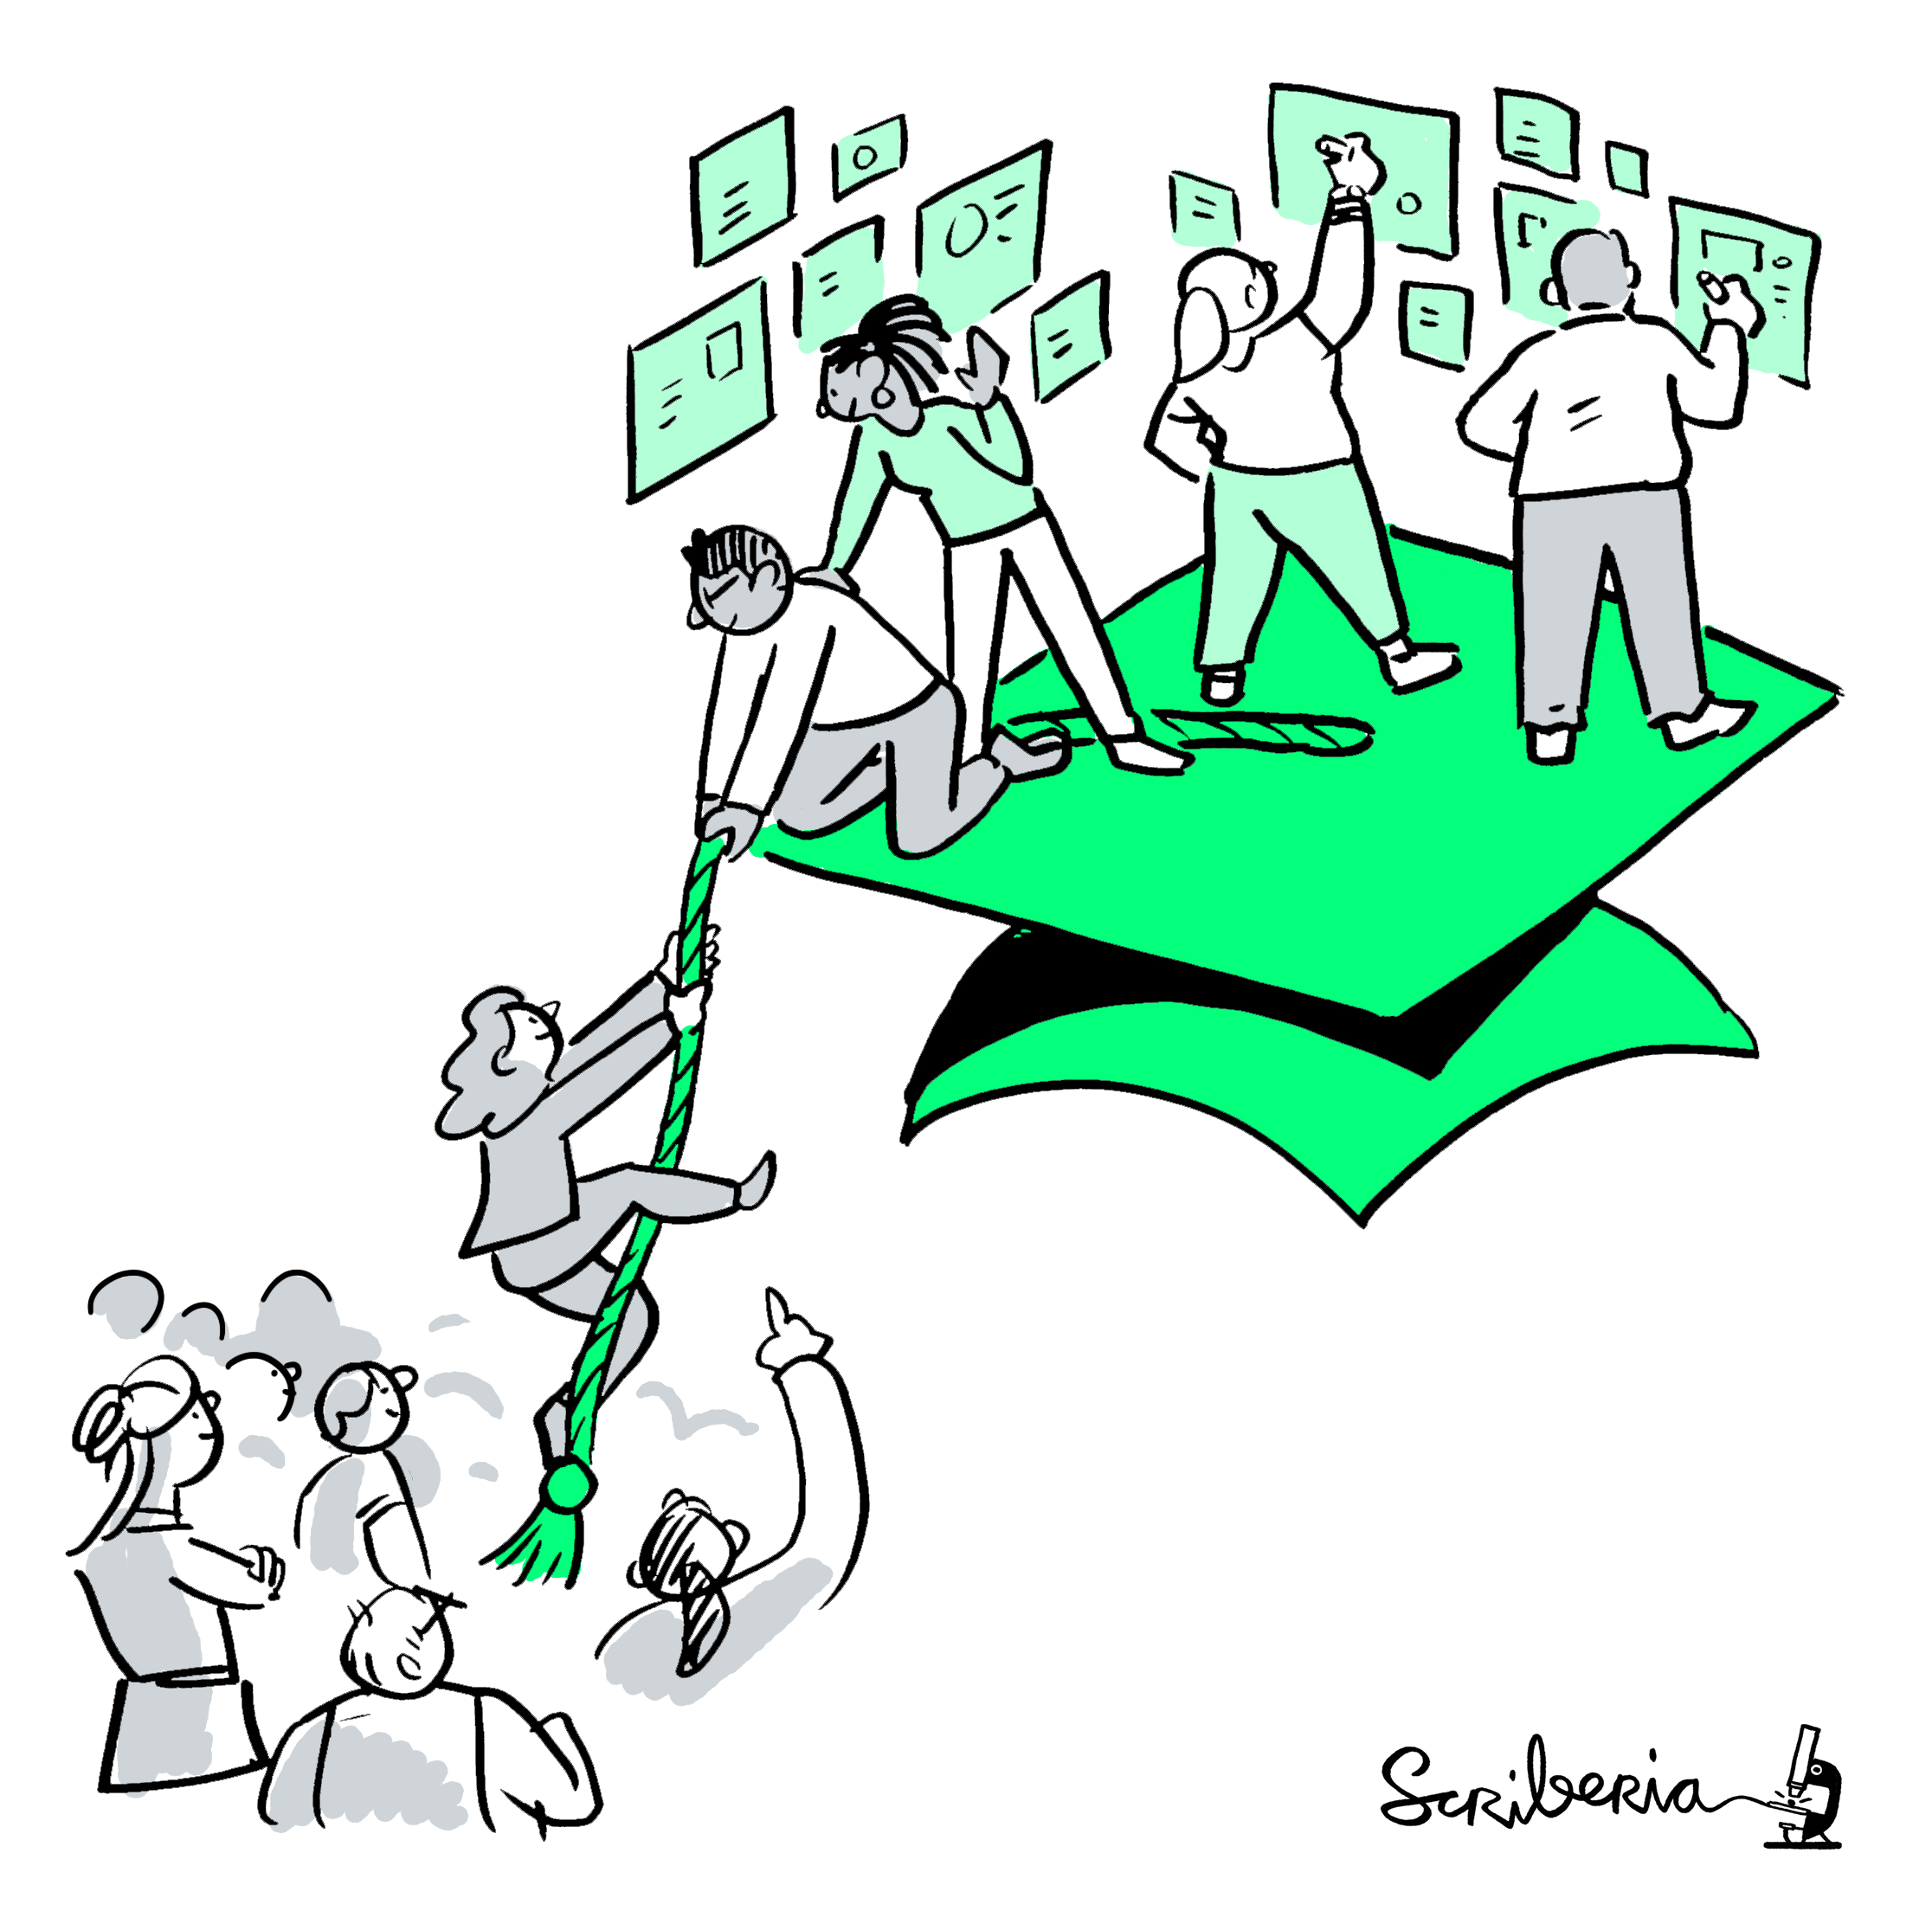
\includegraphics[width=0.5\textwidth]{DecolonisingKnowledge.jpg}
    \end{itemize}
 \end{column}
  \begin{column}{0.2\textwidth}
    \begin{center}
    \begin{itemize}
        \only<2-8>{  
\includegraphics[width=0.4\textwidth]{RStudio_logo.png} \\  }
        \only<2-8>{ \vspace{0.2cm} \hfill 
\includegraphics[width=0.4\textwidth]{git_logo.jpg} \\  }
        \only<2-8>{ \vspace{0.2cm} \includegraphics[width=0.4\textwidth]{github-mark.png} \\  }
        \only<5-8>{ \vspace{0.2cm} \includegraphics[width=0.8\textwidth]{BuildingBlock_rap.png} \\ }
 
    \end{itemize}
    \end{center}
  \end{column}
\end{columns}
\end{frame}


\end{document}

\begin{frame}
\frametitle{Git  \& GitHub}
\begin{center}
    Git \& GitHub are different tools
\end{center}
\begin{columns}[t]
 \begin{column}{0.5\textwidth}
 \begin{itemize}[<+->]
  \item[]{\begin{center}
              
\includegraphics[width=0.2\textwidth]{git_logo.jpg} \\
             \end{center} }
        \item Git is a software
        \item Git needs to be installed
        \item Git works mostly in command mode
        \item Git is complex and unfriendly!

    \end{itemize}
 \end{column}
 \begin{column}{0.5\textwidth}
 \begin{itemize}[<+->]
  \item[]{\begin{center}
              \includegraphics[width=0.4\textwidth]{GitHub-logo.png} \\
             \end{center} }
        \item GitHub is a platform
        \item GitHub needs an account
        \item GitHub can only be accessed remotely
        \item GitHub is (more) friendly
    \end{itemize}
 \end{column}
\end{columns}
\end{frame}


\section{Setup}

\begin{frame}
\frametitle{Setup}

What you'll need to do...
\begin{columns}[t]
 \begin{column}{0.8\textwidth}

 \begin{itemize}[<+->]
        \item Download Git
        \item Install Git on your computer
        \item[$\hookrightarrow$]  Depends on your OS
        \item Create a  GitHub account
        \item Link Git with GitHub account
        \item Link RStudio with Git
        \item[$\hookrightarrow$] May need IT support
        \item[$\hookrightarrow$] Many tutorials exist
    \end{itemize}
 \end{column}
  \begin{column}{0.2\textwidth}
    \begin{center}
    \begin{itemize}
        \only<1-8>{ 
\includegraphics[width=0.6\textwidth]{git_logo.jpg} \\  }
        \only<4-8>{\vspace{0.1 cm} \includegraphics[width=0.95\textwidth]{GitHub-logo.png}  \\  }
        \only<6-8>{ \vspace{0.1cm}  
\includegraphics[width=0.6\textwidth]{RStudio_logo.png} \\  }
    \end{itemize}
    \end{center}
  \end{column}
\end{columns}
\end{frame}

\section{Principles}

\begin{frame}
\frametitle{Principles in action - Overview}
\begin{itemize}
\item[] \textcolor{violet}{\textbf{Alice}} and \textcolor{orange}{\textbf{Bob}} work on the same file\\ \vspace{1cm}
    \only<1>{\includegraphics[width=1.1\textwidth]{GitSimple1.png} \\  }
    \only<2>{\includegraphics[width=1.1\textwidth]{GitSimple2.png} \\  }
    \only<3>{\includegraphics[width=1.1\textwidth]{GitSimple3.png} \\  }
    \only<4>{\includegraphics[width=1.1\textwidth]{GitSimple4.png}   }
\end{itemize}
\end{frame}

\begin{frame}
\frametitle{Important notions}
\begin{columns}[t]
 \begin{column}{0.5\textwidth}
    \begin{itemize}[<+->]
     \item[]
   \begin{center}
    \textcolor{brique}{\textbf{Spaces}}
   \end{center}
    \item  \textcolor{siap}{\textbf{Local working directory:}}
    \item[$\hookrightarrow$] Folder with your file(s)
    \item  \textcolor{siap}{\textbf{Staging area:}}
    \item[$\hookrightarrow$] Local "space" where modified file(s) are stored before commit
    \item \textcolor{siap}{\textbf{Remote repository:}}
    \item[$\hookrightarrow$] Folder  on GitHub platform
    \end{itemize}
 \end{column}
 \begin{column}{0.5\textwidth}
    \begin{itemize}[<+->]
        \item[]
        \begin{center}
        \textcolor{brique}{\textbf{Actions}}
        \end{center}
        \item \textcolor{siap}{\textbf{Commit:}}
        \item[$\hookrightarrow$] A snapshot of file changes
        \item \textcolor{siap}{\textbf{Commit message:}}
        \item[$\hookrightarrow$] A concise description of the changes made
        \item \textcolor{siap}{\textbf{Push:}}
        \item[$\hookrightarrow$] Action of sending modified file(s) to GitHub
        \item \textcolor{siap}{\textbf{Pull:}}
        \item[$\hookrightarrow$] Action of retrieving modified file(s) to local working directory


    \end{itemize}
 \end{column}
\end{columns}
\end{frame}


\begin{frame}
\frametitle{Principles in action - Details}
\textcolor{violet}{\textbf{Alice}} and \textcolor{orange}{\textbf{Bob}} work on the same file (Details)
\pause
\begin{itemize}
\item[]
\only<1>{\includegraphics[width=1.0\textwidth]{GitPrinciple1.png} \\ }
\only<2>{\includegraphics[width=1.0\textwidth]{GitPrinciple2.png} \\ }
\only<3>{\includegraphics[width=1.0\textwidth]{GitPrinciple3N.png} \\ }
\only<4>{\includegraphics[width=1.0\textwidth]{GitPrinciple4N.png} \\ }
\only<5>{\includegraphics[width=1.0\textwidth]{GitPrinciple5N.png} \\ }
\only<6>{\includegraphics[width=1.0\textwidth]{GitPrinciple5N.png} \\ }
\only<7>{\includegraphics[width=1.0\textwidth]{GitPrinciple7N.png} \\ }
\only<8>{\includegraphics[width=1.0\textwidth]{GitPrinciple8N.png} \\ }
\only<9>{\includegraphics[width=1.0\textwidth]{GitPrinciple9N.png} \\ }
\only<10>{\includegraphics[width=1.0\textwidth]{GitPrinciple10N.png} \\ }
\only<11>{\includegraphics[width=1.0\textwidth]{GitPrinciple11N.png} \\ }
\only<12>{\includegraphics[width=1.0\textwidth]{GitPrinciple12N.png} \\ }
\only<13>{\includegraphics[width=1.0\textwidth]{GitPrinciple13N.png} \\ }
\end{itemize}
\end{frame}

\section{Issues}

\begin{frame}
\frametitle{Remarks and issues}
    \begin{itemize}[<+->]
     \item A commit can include changes from multiple files simultaneously
     \item One can do several commits before pushing (to GitHub)
     \item Commit messages can be edited (\texttt{amend})
     \item Every commit has an identifier (\texttt{hash} or \texttt{SHA})
     \item Git manage complex situations
     \item Only a few actions available in RStudio
    \end{itemize}
\end{frame}

\begin{frame}
\frametitle{Principles in action - Complex situations}
\textcolor{violet}{\textbf{Alice}} and \textcolor{orange}{\textbf{Bob}} work on the same file \textbf{at the same time}
\pause
\begin{itemize}
\item[]
\only<1>{\includegraphics[width=1.0\textwidth]{GitComplex2N.png} \\ }
\only<2>{\includegraphics[width=1.0\textwidth]{GitComplex2N.png} \\ }
\only<3>{\includegraphics[width=1.0\textwidth]{GitComplex3N.png} \\ }
\only<4>{\includegraphics[width=1.0\textwidth]{GitComplex4N.png} \\ }
\only<5>{\includegraphics[width=1.0\textwidth]{GitComplex5N.png} \\ }
\only<6>{\includegraphics[width=1.0\textwidth]{GitComplex6N.png} \\ }
\only<7>{\includegraphics[width=1.0\textwidth]{GitComplex7N.png} \\ }
\only<8>{\includegraphics[width=1.0\textwidth]{GitComplex8N.png} \\ }
\only<9>{\includegraphics[width=1.0\textwidth]{GitComplex9N.png} \\ }
\only<10>{\includegraphics[width=1.0\textwidth]{GitComplex10N.png} \\ }
\end{itemize}
\end{frame}


\section{Takeaways}

\begin{frame}
\frametitle{Takeaways}
 Git:
\begin{itemize}[<+->]
    \item Tracks files changes over time
    \item[$\hookrightarrow$] Changes can be visualized
    \item Facilitates team collaboration  and file sharing
    \item Manages complex situations of simultaneous changes
    \item Works well with GitHub \& Rstudio
    \item[$\hookrightarrow$] Advanced operations need line command instructions \\
    \includegraphics[width=0.7\textwidth]{GitPrompt.png} \\
    \end{itemize}
\end{frame}

\begin{frame}
\frametitle{To conclude}
\begin{columns}[t]
 \begin{column}{0.5\textwidth}
    \begin{itemize}[<+->]
    \item Git can be challenging!
    \item Learning Git takes time
    \item Simple operations easy to use
    \item[$\hookrightarrow$] Work in teams

    \end{itemize}
 \end{column}
 \begin{column}{0.5\textwidth}
    \begin{itemize}
    \item[]
    \only<1-6>{\includegraphics[width=0.6\textwidth]{GitError1.png} \\ }
    \only<1-6>{\hfill \includegraphics[width=0.6\textwidth]{GitError2.png} \\ }
    \only<1-6>{\includegraphics[width=0.6\textwidth]{GitError3.png} \\ }
    \end{itemize}
 \end{column}
\end{columns}
 \begin{itemize}[<+->]
 \item[]
    \item[]
    \begin{center}
    Installing/working with Git \\
     \textbf{is not mandatory} for this course
    \end{center}
  \end{itemize}
\end{frame}


\end{document}


 \only<1>{\includegraphics[width=1.0\textwidth]{GitPrinciple1.png} \\
 \only<2>{\includegraphics[width=1.0\textwidth]{GitPrinciple2.png} \\
 \only<3>{\includegraphics[width=1.0\textwidth]{GitPrinciple3.png} \\
 \only<4>{\includegraphics[width=1.0\textwidth]{GitPrinciple4.png} \\
 \only<5>{\includegraphics[width=1.0\textwidth]{GitPrinciple5.png} \\
 \only<6>{\includegraphics[width=1.0\textwidth]{GitPrinciple6.png} \\
 \only<7>{\includegraphics[width=1.0\textwidth]{GitPrinciple7.png} \\
 \only<8>{\includegraphics[width=1.0\textwidth]{GitPrinciple8.png} \\
 \only<9>{\includegraphics[width=1.0\textwidth]{GitPrinciple9.png} \\
 \only<10>{\includegraphics[width=1.0\textwidth]{GitPrinciple10.png} \\
 \only<11>{\includegraphics[width=1.0\textwidth]{GitPrinciple11.png} \\
 \only<12>{\includegraphics[width=1.0\textwidth]{GitPrinciple12.png} \\
 \only<13>{\includegraphics[width=1.0\textwidth]{GitPrinciple13.png} \\
 \only<14>{\includegraphics[width=1.0\textwidth]{GitPrinciple14.png} \\
 \only<15>{\includegraphics[width=1.0\textwidth]{GitPrinciple15.png} \\
 \only<16>{\includegraphics[width=1.0\textwidth]{GitPrinciple16.png} \\
 \only<17>{\includegraphics[width=1.0\textwidth]{GitPrinciple17.png} \\
 \only<18>{\includegraphics[width=1.0\textwidth]{GitPrinciple18.png} \\
 \only<19>{\includegraphics[width=1.0\textwidth]{GitPrinciple19.png} \\


\end{document}


%%%%%%%%%%%%%%% Last Slide %%%%%%%%%%%%%%%%

\begin{frame}[allowframebreaks]%in case more than 1 slide needed
\frametitle{References}
    {\footnotesize
    %\bibliographystyle{authordate1}
    \bibliographystyle{apalike}
    \bibliography{c:/Chris/Visualisation/Visu}
    }
\end{frame}


%\bibliographystyle{authordate1}
%\bibliography{c:/Chris/Visualisation/Visu}
%\end{frame}

\begin{frame} % Cover slide
\frametitle{ }
\pause
 \begin{itemize}[<+->]
  \item[]
  \item
\end{itemize}
\end{frame}
